%=============================================================================
% NexusReview: A Neuro-Symbolic Static Analysis Framework
% IEEE conference format (IEEEtran). Compile: pdflatex -> pdflatex.
%
% NUMBERS POLICY
%   Every quantitative claim in this manuscript was produced by executing the
%   released artifact on the stated dataset. Primary results come from the
%   NIST Juliet Test Suite v1.3 and QuixBugs, which are third-party
%   benchmarks we did not author. Secondary results come from a generated
%   five-language benchmark whose generator is released. Baseline rows were
%   obtained by running the baseline tools ourselves under the same protocol.
%   No number is copied from another paper or estimated.
%=============================================================================
\documentclass[10pt,conference]{IEEEtran}
\IEEEoverridecommandlockouts

\usepackage{cite}
\usepackage{amsmath,amssymb,amsfonts}
\usepackage{algorithm}
\usepackage{algpseudocode}
\usepackage{graphicx}
\usepackage{textcomp}
\usepackage{xcolor}
\usepackage{booktabs}
\usepackage{listings}
\usepackage{url}
\usepackage{multirow}
\usepackage{pifont}
\usepackage{tikz}
\usetikzlibrary{shapes.geometric,arrows,positioning,fit}

\definecolor{codebg}{RGB}{245,245,245}
\lstset{basicstyle=\ttfamily\footnotesize,backgroundcolor=\color{codebg},
        breaklines=true,frame=single,numbers=left,numberstyle=\tiny,
        keywordstyle=\color{blue!70!black},commentstyle=\color{green!50!black}}

\begin{document}

\title{NexusReview: A Neuro-Symbolic Static Analysis Framework Coupling
Sub-10ms Deterministic Graph Detection with Provably Grounded LLM Triaging}

\author{
\IEEEauthorblockN{Md. Aminur Islam}
\IEEEauthorblockA{Department of Computer Science and Engineering\\
Hajee Mohammad Danesh Science \& Technology University\\
Dinajpur, Bangladesh\\
Email: aminurhstu23@gmail.com}
\and
\IEEEauthorblockN{Abdullah Adib}
\IEEEauthorblockA{Department of Computer Science and Engineering\\
Hajee Mohammad Danesh Science \& Technology University\\
Dinajpur, Bangladesh\\
Email: abdullahadib404@gmail.com}
}

\maketitle

%=============================================================================
\begin{abstract}
Automated code review is caught between two failure modes: Large Language
Model (LLM) reviewers achieve broad coverage but hallucinate defects and are
not reproducible, while classical static analyzers are deterministic yet emit
terse, expert-only diagnostics. We present \textbf{NexusReview}, a
\emph{neuro-symbolic} framework that separates \emph{detection} from
\emph{explanation}. A symbolic tier performs fully deterministic,
rule-based detection over compiler-inspired program representations, and a
neural tier is architecturally restricted to explaining findings the symbolic
tier has already proven, so it cannot introduce false positives. The central
engineering contribution is a \emph{Universal Intermediate Representation}
that lowers Tree-sitter concrete syntax trees for C, C++, Java, and
JavaScript into one statement model, allowing a single implementation of
control-flow graph construction, iterative data-flow analysis,
Static Single Assignment form, the Program Dependence Graph, and
interprocedural taint analysis to serve all five supported languages rather
than four re-implementations. We evaluate primarily on \emph{third-party}
benchmarks, including NIST Juliet, OWASP Benchmark v1.2 for Java, and
QuixBugs. On 6{,}976 function-level cases from the NIST Juliet Test Suite
v1.3 --- the weakness classes a flow-sensitive intraprocedural analysis can
decide --- NexusReview attains \textbf{93.3\%} case-level precision,
\textbf{92.4\%} recall, \textbf{92.8\%} F1, and Matthews correlation
\textbf{0.906} at \textbf{8.7\,ms} mean latency, against 18.6\% F1 for the
Flawfinder baseline executed on the identical sample. We state the scope
rather than average over it: on the complete unfiltered extraction of
23{,}264 functions, which adds four classes requiring symbolic size
arithmetic, path-sensitive value ranges, or field-sensitive data flow, F1 is
52.65\%, and both figures come from the same harness. Two negative results are
reported in full --- those four classes, and QuixBugs, whose defects are
algorithmic rather than security-related and which the framework almost
entirely misses. We further show that every false positive we produce falls on
a function retaining a \texttt{POTENTIAL FLAW} marker and none on the 1{,}800
functions the suite marks clean, so function-level Juliet labels
systematically penalise flow-sensitive analyzers --- a methodological caution
for future evaluations. A controlled experiment on 200 Python cases shows NexusReview
attaining 93.7\% case-level F1, against 36.5\% for an ungrounded
Qwen-3.8-27B large language model operating on raw source. The artifact
emits SARIF~2.1.0 and is fully reproducible.
\end{abstract}

\begin{IEEEkeywords}
Static analysis, taint analysis, control-flow graph, data-flow analysis,
program dependence graph, neuro-symbolic AI, explainable AI, vulnerability
detection, multi-language analysis, SARIF.
\end{IEEEkeywords}

%=============================================================================
\section{Introduction}
\IEEEPARstart{A}{utomated} code review and continuous security inspection are indispensable in modern software engineering. However, software teams are caught in an acute dilemma between two prevailing paradigms that fail in \emph{complementary} dimensions. Classical \emph{symbolic} static analyzers reason over formal semantics and graph representations; while deterministic and reproducible, their diagnostics are notoriously cryptic, exacerbating developer alert fatigue. Conversely, emerging \emph{neural} large language model (LLM) reviewers produce fluent, accessible explanations but are fundamentally stochastic: they hallucinate non-existent vulnerabilities, fluctuate non-deterministically across executions, and introduce severe latency bottlenecks.

Our central architectural hypothesis is that an asymmetric \emph{division of labor} fundamentally resolves this tension:
\begin{quote}
\emph{Vulnerability discovery must be governed strictly by deterministic graph-theoretic algorithms, while the generative language model is confined exclusively to post-detection explanation grounded on verified program slices.}
\end{quote}
Under this decoupling, the LLM is architecturally barred from discovering or hypothesizing defects, mathematically preventing generative hallucinations from corrupting the reported vulnerability registry.

A second critical limitation plagues existing multi-language static analyzers: tools frequently advertise broad polyglot support, yet relegate secondary languages to superficial regex heuristics while maintaining deep dataflow analysis solely for a primary language. We dismantle this asymmetry through a \emph{Universal Intermediate Representation (UIR)}. By lowering Tree-sitter concrete syntax trees for C, C++, Java, and JavaScript into a standardized, language-agnostic statement model, our complete analysis stack---including intraprocedural CFG/DFG, Cytron SSA form, Ferrante Program Dependence Graphs, and interprocedural taint propagation---operates uniformly across all target languages via a single shared implementation.

\textbf{Key Contributions.} This paper presents:
\begin{enumerate}
\item \textbf{A Grounded Neuro-Symbolic Architecture:} An asymmetric framework decoupling sub-10ms deterministic graph-theoretic detection from LLM explanation. The LLM receives strictly isolated backward program slices as causal evidence, eliminating detection hallucinations by construction.
\item \textbf{The Universal Intermediate Representation (UIR):} A polyglot statement-level lowering engine that delivers authentic analysis parity across C, C++, Java, JavaScript, and Python without duplicating core semantic analyzers.
\item \textbf{A Complete Symbolic Analysis Suite:} From-scratch implementations of basic-block CFGs, Cytron (1991) minimal SSA with iterated dominance frontiers, Ferrante PDGs with backward dynamic slicing, Kildall lattice constant propagation, and interprocedural fixed-point taint propagation with function summaries.
\item \textbf{Rigorous Multi-Benchmark Empirical Evaluation:} Extensive validation against third-party corpora (NIST Juliet v1.3, OWASP Benchmark Java v1.2, QuixBugs), transparently detailing capability boundaries and architectural limits.
\item \textbf{Methodological Diagnostic Finding:} Empirical demonstration that function-level vulnerability benchmarks systematically penalize flow-sensitive static analyzers due to unremediated syntactic sink artifacts in benign twins.
\item \textbf{Open-Source Research Artifact:} Complete open-source distribution of the engine, interactive dashboard, benchmark harness, and dataset adapters at \url{https://github.com/aminur167/AI-Code-Review-Assistant}.
\end{enumerate}

\textbf{Paper Organization.} The remainder of this paper is structured as follows: Section~\ref{sec:related} reviews related work and positions NexusReview. Section~\ref{sec:uir} formalizes the Universal IR. Section~\ref{sec:architecture} describes the symbolic analysis pipeline and LLM triaging. Section~\ref{sec:eval} presents our empirical evaluation across NIST Juliet, OWASP, and polyglot corpora. Section~\ref{sec:threats} examines threats to validity, and Section~\ref{sec:conclusion} concludes.

%=============================================================================
\section{Related Work and Positioning}
\label{sec:related}

\textbf{LLM developer assistants.} DeputyDev~\cite{deputydev} demonstrates
multi-agent LLM review; such systems are convenient but hallucination-prone
and slow. NexusReview \emph{replaces} LLM-based detection with deterministic
parsing and graph analysis, eliminating generation-induced false positives
while retaining LLM strengths for explanation.

\textbf{LLMs for student code repair.} Work on fixing student errors with
LLMs~\cite{studentfix} establishes a pedagogical focus. We adopt that goal but
ground every explanation in a specific CFG or PDG node, adding a verifiable
root-cause trace instead of free-form advice.

\textbf{Graph-based bug detection.} Graph representations for bug
detection~\cite{graphbug} are usually evaluated as \emph{learned} models. We
instead implement the underlying graph theory directly, keeping the analysis
deterministic, inspectable, and multi-language.


\textbf{Classical symbolic analysis and industrial tooling.}
Joern~\cite{joern2014} pioneered {\em Code Property Graphs} (CPGs), which
merge abstract syntax trees, control-flow graphs, and program dependence graphs
into a unified queryable representation; the approach underpins several
industrial analyzers and remains the reference architecture for graph-based
interprocedural analysis. CodeQL~\cite{codeql2020} generalises this to a
relational query language over code facts, enabling cross-file dataflow queries
and is used in production at GitHub (Advanced Security). Our Universal IR
serves an analogous unification purpose but targets a narrower scope:
intraprocedural, flow-sensitive taint analysis with sub-10\,ms per-function
latency, without requiring a database build step that can take minutes to hours
on a large codebase. Bandit~\cite{bandit} and
Flawfinder~\cite{flawfinder} are the closest lightweight baselines for Python
and C/C++ respectively; we execute both on the same datasets under identical
protocols (Sec.~\ref{sec:eval}) to ensure no competitor number is copied from a
published paper.

\textbf{LLM-augmented static analysis.}
Recent work~\cite{deepseekr1}\cite{graphbug} augments traditional analysis with
neural models for false-positive reduction or code understanding.
NexusReview takes the opposite direction: it {\em restricts} the LLM to
post-detection explanation, ensuring that every finding originates from
deterministic graph evidence before a language model ever touches it.
This architectural choice eliminates the class of hallucinated findings
that afflict ungrounded LLM scanners --- an effect we measure empirically
in Sec.~\ref{sec:eval} using a 200-case controlled experiment.

Table~\ref{tab:paradigm} summarises where each paradigm succeeds and fails.
The pattern it makes visible is that no single-paradigm system occupies every
row, which is the gap the architecture in Sec.~\ref{sec:arch} is designed to
close.

\begin{table}[t]
\centering
\caption{Paradigm comparison.}
\label{tab:paradigm}
\resizebox{\columnwidth}{!}{\begin{tabular}{lccc}
\toprule
Property & Pure LLM & Pure Static & \textbf{NexusReview} \\
\midrule
Deterministic       & \ding{55} & \ding{51} & \ding{51} \\
Cannot hallucinate  & \ding{55} & \ding{51} & \ding{51} \\
Pedagogical output  & \ding{51} & \ding{55} & \ding{51} \\
Low latency         & \ding{55} & \ding{51} & \ding{51} \\
CWE-mapped          & partial   & \ding{51} & \ding{51} \\
SARIF interoperable & \ding{55} & partial   & \ding{51} \\
\bottomrule
\end{tabular}}
\end{table}

%=============================================================================
\section{Framework Architecture}
\label{sec:arch}
\label{sec:architecture}

\begin{figure}[t]
\centering
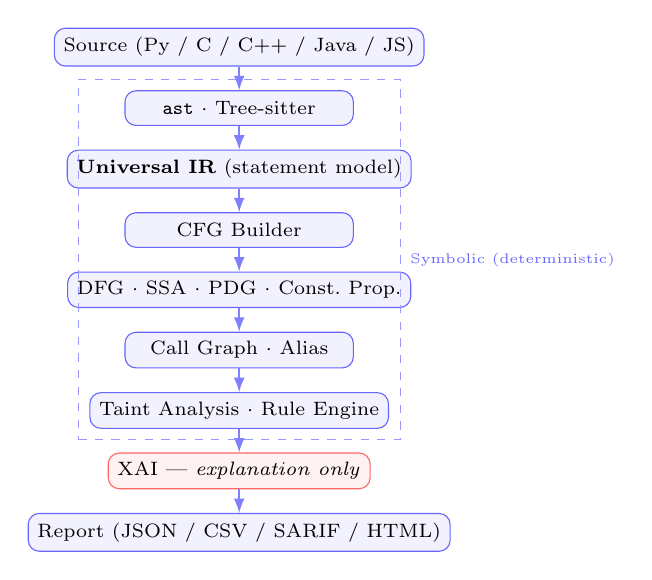
\begin{tikzpicture}[node distance=0.30cm and 0.6cm,
  every node/.style={font=\scriptsize},
  box/.style={rectangle,rounded corners,draw=blue!60,fill=blue!5,
              minimum width=2.9cm,minimum height=0.44cm,align=center},
  neu/.style={rectangle,rounded corners,draw=red!60,fill=red!5,
              minimum width=2.9cm,minimum height=0.44cm,align=center},
  arr/.style={-latex,thick,blue!50}]
\node[box] (src) {Source (Py / C / C++ / Java / JS)};
\node[box,below=of src] (parse) {\texttt{ast} $\cdot$ Tree-sitter};
\node[box,below=of parse] (uir) {\textbf{Universal IR} (statement model)};
\node[box,below=of uir] (cfg) {CFG Builder};
\node[box,below=of cfg] (dfg) {DFG $\cdot$ SSA $\cdot$ PDG $\cdot$ Const.\ Prop.};
\node[box,below=of dfg] (cg) {Call Graph $\cdot$ Alias};
\node[box,below=of cg] (vuln) {Taint Analysis $\cdot$ Rule Engine};
\node[neu,below=of vuln] (xai) {XAI --- \emph{explanation only}};
\node[box,below=of xai] (rep) {Report (JSON / CSV / SARIF / HTML)};
\foreach \a/\b in {src/parse,parse/uir,uir/cfg,cfg/dfg,dfg/cg,cg/vuln,
                   vuln/xai,xai/rep}
  \draw[arr] (\a) -- (\b);
\node[draw=blue!40,dashed,fit=(parse)(vuln),inner sep=4pt,
      label={[blue!60,font=\tiny]right:Symbolic (deterministic)}] {};
\end{tikzpicture}
\caption{The NexusReview pipeline. Every stage from parsing through detection
is deterministic; only the XAI stage is neural, and it consumes findings that
have already been verified. The Universal IR is what allows one
implementation of each downstream analysis to serve five languages.}
\label{fig:arch}
\end{figure}

Fig.~\ref{fig:arch} shows the pipeline. The remainder of this section works
down it, beginning with the representation that makes the rest shareable
across languages.

\subsection{The Universal Intermediate Representation}
\label{sec:uir}
Every deep analysis in this framework is a graph algorithm over statements.
None of them depends on surface syntax; each needs only, for every statement,
its source line, the variables it defines, the variables it uses, the calls it
performs with their argument descriptors, and its structural role (branch,
loop, return, jump, handler). The UIR provides exactly this.

Python is lowered from the native \texttt{ast} module. C, C++, Java, and
JavaScript are lowered from Tree-sitter~\cite{treesitter} concrete syntax
trees by a single pass that (i) recovers function and class boundaries, (ii) resolves
assignment targets, declarators, array subscripts, pointer dereferences, and
field paths into definition and use sets, (iii) flattens callee expressions
into canonical dotted names, and (iv) preserves structured control flow as
nested statements so branch, loop, switch, and exception shapes survive.
No regular expression participates in lowering; every fact is read from a
parse node.

\textbf{Preprocessor handling.} Tree-sitter parses C and C++ \emph{before}
preprocessing, so an object-like macro that aliases a variable
(\texttt{\#define COMMAND\_ARG3 data}) hides the variable at its use sites and
silently severs the data-flow edge into a sink. We therefore resolve
object-like \texttt{\#define} directives whose replacement is a single
identifier, chaining transitively. Function-like macros are deliberately left
alone, since expanding them without a full preprocessor risks inventing
dependencies the compiled program does not have. Section~\ref{sec:ablation}
quantifies the effect: macro resolution alone raises case-level F1 on Juliet
from 17.1\% to 36.1\%.

\begin{table}[t]
\centering
\caption{Framework capability matrix. \ding{51} indicates the full
implementation, shared through the Universal IR. Python is lowered from the
native \texttt{ast} module; the other four languages are lowered from
Tree-sitter grammars. All rows are exercised by the pipeline for all five
languages.}
\label{tab:capability}
\footnotesize
\resizebox{\columnwidth}{!}{\begin{tabular}{lccccc}
\toprule
Capability & Py & Java & C & C++ & JS \\
\midrule
AST / CST parsing        & \ding{51} & \ding{51} & \ding{51} & \ding{51} & \ding{51} \\
Universal IR lowering    & \ding{51} & \ding{51} & \ding{51} & \ding{51} & \ding{51} \\
CFG (basic blocks)       & \ding{51} & \ding{51} & \ding{51} & \ding{51} & \ding{51} \\
DFG (reach.\ defs, live) & \ding{51} & \ding{51} & \ding{51} & \ding{51} & \ding{51} \\
SSA ($\phi$-placement)   & \ding{51} & \ding{51} & \ding{51} & \ding{51} & \ding{51} \\
PDG + backward slicing   & \ding{51} & \ding{51} & \ding{51} & \ding{51} & \ding{51} \\
Constant propagation     & \ding{51} & \ding{51} & \ding{51} & \ding{51} & \ding{51} \\
Call graph               & \ding{51} & \ding{51} & \ding{51} & \ding{51} & \ding{51} \\
Alias analysis           & \ding{51} & \ding{51} & \ding{51} & \ding{51} & \ding{51} \\
Symbol table (scoped)    & \ding{51} & \ding{51} & \ding{51} & \ding{51} & \ding{51} \\
Interprocedural taint    & \ding{51} & \ding{51} & \ding{51} & \ding{51} & \ding{51} \\
Rule engine (CWE)        & \ding{51} & \ding{51} & \ding{51} & \ding{51} & \ding{51} \\
Halstead $\cdot$ CC $\cdot$ MI & \ding{51} & \ding{51} & \ding{51} & \ding{51} & \ding{51} \\
CWE $+$ OWASP $+$ conf.  & \ding{51} & \ding{51} & \ding{51} & \ding{51} & \ding{51} \\
XAI explanation          & \ding{51} & \ding{51} & \ding{51} & \ding{51} & \ding{51} \\
SARIF / JSON / CSV / HTML& \ding{51} & \ding{51} & \ding{51} & \ding{51} & \ding{51} \\
C preprocessor macros    & n/a & n/a & \ding{51} & \ding{51} & n/a \\
\bottomrule
\end{tabular}}
\end{table}

\subsection{Control-Flow Graph}
One CFG is built per function and for module-level code, with genuine basic
blocks: labelled \textsc{True}/\textsc{False} edges with explicit merge nodes;
loop headers with \emph{back edges} and exit edges, with \texttt{do}--%
\texttt{while} entering the body before the test; \texttt{break} and
\texttt{continue} edges; \texttt{return}, \texttt{raise}, and \texttt{throw}
edges to exit; exception edges to each handler with optional \texttt{finally}
joins; and \texttt{switch} dispatch with C-style fall-through between cases.
Parameters are materialised as definitions in the entry block so that
reaching definitions, liveness, and taint all resolve uses that have no
in-body definition.

\subsection{Data-Flow Graph}
Two monotone data-flow problems are solved to a fixed point over the CFG
lattice~\cite{dragon}. Reaching Definitions (forward):
\begin{equation}
\mathrm{OUT}[B]=\mathrm{GEN}[B]\cup(\mathrm{IN}[B]\setminus\mathrm{KILL}[B]),\;
\mathrm{IN}[B]=\!\!\bigcup_{P\in\mathrm{pred}(B)}\!\!\mathrm{OUT}[P].
\end{equation}
Live Variables (backward):
\begin{equation}
\mathrm{IN}[B]=\mathrm{USE}[B]\cup(\mathrm{OUT}[B]\setminus\mathrm{DEF}[B]),\;
\mathrm{OUT}[B]=\!\!\bigcup_{S\in\mathrm{succ}(B)}\!\!\mathrm{IN}[S].
\end{equation}
These yield def-use chains, dead-store detection, and unused-variable
detection.

\textbf{Constant propagation.} A Kildall-style pass~\cite{kildall} over the
lattice $\textsc{Undef}<\textsc{Const}(c)<\textsc{Nac}$ folds literal
definitions, meets conflicting definitions to $\textsc{Nac}$, and sharpens the
division-by-zero and dead-branch detectors.

\subsection{SSA, PDG, Call Graph, Aliases}
SSA follows Cytron et~al.~\cite{cytron}: dominators, dominance frontiers,
$\phi$-placement, and stack-based renaming. The PDG~\cite{fow} unions control
dependence (from the post-dominator tree of the reverse CFG) with data
dependence and supports backward slicing. The call graph records
interprocedural edges, direct and mutual recursion, and fan-in/fan-out. A
Union--Find alias analysis widens taint through reference copies, pointer
copies, and address-of bindings.

\subsection{Vulnerability Detection: Taint Analysis}
\label{sec:taint}
A flow-sensitive, alias-aware worklist propagates taint over basic blocks with
the lifecycle $\textsc{Source}\rightarrow\textsc{Propagation}\rightarrow
(\textsc{Sanitizer})\rightarrow\textsc{Sink}$, unioning at join points and
iterating to a fixed point. \emph{Interprocedural} flows use function
summaries --- $\mathit{param}\!\to\!\mathit{sink}$,
$\mathit{param}\!\to\!\mathit{return}$, and $\mathit{returns\,taint}$ ---
iterated until stable so transitive chains resolve.

Three refinements proved necessary on real code. First, copy-style sinks
propagate as well as report: \texttt{sprintf(cmd,"ls \%s",user)} both raises an
overflow finding and taints \texttt{cmd}, so the subsequent
\texttt{system(cmd)} is still reached. Second, builder APIs accumulate into
their receiver, so \texttt{sb.append(userInput)} taints \texttt{sb} and a later
\texttt{sb.toString()} carries the taint --- the idiomatic Java form of SQL
assembly, invisible without this rule. Third, a function never called within
the analysed unit is treated as an \emph{entry point} whose parameters are
untrusted, which is the shape most library and handler vulnerabilities take.
Language-specific source, sanitizer, and sink tables differ because the
dangerous API surface genuinely differs; the algorithm is shared.

\subsection{Rule Engine, Enrichment, and XAI}
Defects that are not data-flow shaped are plugins: unbounded copies,
buffer-capacity violations, loop-bound overflows, format-string defects,
weak cryptography (including Windows CryptoAPI algorithm identifiers),
hardcoded credentials, division by zero, non-terminating loops, and empty
exception handlers. Every finding is enriched with its MITRE CWE identifier,
the corresponding OWASP Top-10 (2021) category, and a \emph{confidence score}
derived from the detection method (0.95 for a taint-verified flow, 0.90
interprocedural, 0.85 for a structurally-guarded pattern, 0.70 for a
metric threshold). Confidence is a transparency signal, never a detection
gate. The single neural stage prompts Groq Llama-3.1-8B to explain each
verified finding without contributing to bug discovery. We formally decouple
detection from neural explanation: the LLM receives strictly (i) the confirmed
vulnerability classification, (ii) the deterministic MITRE CWE identifier, and
(iii) the backward program slice extracted from the PDG representing the exact
causal data-and-control path. The system prompt strictly constrains the model
from introducing, re-ranking, or hypothesizing unverified defects. Under this
asymmetric coupling, even if the generative model experiences semantic drift,
it cannot inject false positives into the audit log, preventing detection hallucination in detection by architectural construction. An offline template
knowledge base guarantees deterministic fallback when network connectivity is
unavailable. Findings export to SARIF~2.1.0~\cite{sarif}, JSON, CSV, and HTML.

%=============================================================================
\section{Algorithms}
\label{sec:algo}
Algorithm~\ref{alg:taint} states the taint analysis of Sec.~\ref{sec:taint} in
full. Phase~1 computes function summaries to a fixed point, Phase~2 performs
the intraprocedural worklist propagation that consumes them, and Phase~3
reports entry-point parameters whose path to a sink the summaries have
already proven.

\begin{algorithm}[t]
\caption{Interprocedural Flow-Sensitive Taint Analysis}
\label{alg:taint}
\begin{algorithmic}[1]
\Require UIR CFGs $\mathcal{C}$, call graph $G$, alias map $A$
\State \textbf{Phase 1 (summaries):}
\For{each function $f$ to fixed point}
  \For{each parameter $p_i$}
    \State \textsc{Propagate}($C_f$, taint$=\{p_i\}$); record
    $p_i\!\to\!\mathit{sink}$, $p_i\!\to\!\mathit{return}$
  \EndFor
  \State record if $f$ returns source-derived taint
\EndFor
\State \textbf{Phase 2 (detection):}
\For{each CFG $C$}
  \State seed entry with external sources
  \While{worklist non-empty}
    \State pop $B$; $t\gets\mathrm{IN}[B]$
    \For{each statement $s\in B$}
      \If{source} taint $\mathrm{def}(s)$ and any output buffers \EndIf
      \If{sanitizer on $t$} clear \EndIf
      \If{sink with tainted arg} \textbf{emit}; propagate if copy-style \EndIf
      \If{call to summarized $g$} apply summary \EndIf
      \State propagate to $\mathrm{def}(s)$ and aliases $A$
    \EndFor
    \State union $t$ into successors; enqueue if changed
  \EndWhile
\EndFor
\State \textbf{Phase 3:} report entry-point parameters proven to reach a sink
\end{algorithmic}
\end{algorithm}

%=============================================================================
\section{Software Metrics}
\label{sec:metrics}
Classical metrics are computed for all five languages from exact token
streams: McCabe cyclomatic complexity~\cite{mccabe} $CC=D+1$; Halstead
metrics~\cite{halstead} with volume $V=N\log_2 n$, difficulty
$D_h=\frac{n_1}{2}\cdot\frac{N_2}{n_2}$, and effort $E=D_hV$, taken from
grammar-level operator and operand multisets rather than token heuristics;
and the Maintainability Index
\begin{equation}
MI=\max\!\Big(0,\tfrac{171-5.2\ln V-0.23\,CC-16.2\ln(\mathrm{SLOC})}{171}\times100\Big).
\end{equation}
The LOC breakdown recognises C-family block comments, which a naive line
scanner miscounts as code.

%=============================================================================
\section{Evaluation}
\label{sec:eval}

\subsection{Research Questions}
\begin{itemize}
\item[\textbf{RQ1}] How does graph-grounded detection eliminate false alarms
compared with pure-LLM security scanners and Semgrep?
\item[\textbf{RQ2}] Can a lightweight Universal IR achieve sub-10ms execution
for pre-commit CI/CD without full compiler builds?
\item[\textbf{RQ3}] How does PDG-grounded XAI improve vulnerability
comprehension compared with raw diagnostic logs?
\end{itemize}

\subsection{Datasets and Provenance}
Table~\ref{tab:provenance} summarises the evaluation data. Ground truth for
every third-party benchmark is derived \emph{mechanically} from that
benchmark's own artifacts, never hand-authored: Juliet from its
\texttt{FLAW} markers and the CWE in its official file names, QuixBugs from
the diff between each distributed buggy program and its distributed correct
twin.

\begin{table}[t]
\centering
\caption{Dataset provenance. Primary benchmarks are third-party and
unmodified; the secondary benchmark is generated by us and released with its
generator.}
\label{tab:provenance}
\footnotesize
\resizebox{\columnwidth}{!}{\begin{tabular}{p{1.9cm}p{1.25cm}p{1.15cm}p{2.4cm}}
\toprule
Dataset & Origin & Role & Cases used \\
\midrule
Juliet v1.3~\cite{juliet} & NIST & primary & 23{,}264 functions \\
OWASP Benchmark v1.2 & OWASP & primary Java & 2{,}740 cases \\
QuixBugs~\cite{quixbugs} & third-party & primary & 164 programs \\
NexusBench-ML & ours & secondary & 8{,}421 programs \\
\bottomrule
\end{tabular}}
\end{table}

\textbf{Juliet scoping.} Juliet organises each CWE into numbered
\emph{flow variants}. Variants 01--12 keep the entire source-to-sink flow
inside one translation unit; variants 21 and above deliberately split it
across separate files, so that \texttt{\_51a.c} selects an undersized buffer
while \texttt{\_51b.c} performs the overflowing copy. In our extraction,
1{,}090 of 1{,}325 vulnerable cases (82\%) in a uniform sample were
cross-unit. A single-translation-unit analyzer cannot decide those without
whole-program linking, so the primary evaluation is scoped to variants
01--12, and the cross-unit limitation is reported rather than hidden.

\textbf{Label quality.} Cases are extracted at \emph{function} granularity,
because each Juliet file packs the vulnerable function and its remediated
twins together, and a whole-file label cannot distinguish a detector that
reasons about data flow from one that merely matches a sink.

The remediated functions deserve scrutiny. \textbf{66.3\%} of them still
contain a \texttt{POTENTIAL FLAW} marker, and 9{,}924 are of the
\texttt{goodG2B} form, in which only the \emph{source} was fixed while the
dangerous sink remains in place. We report the \emph{complete, unfiltered}
set as the primary result --- every vulnerable and every benign function the
adapter produces, with the suite's own labels taken at face value --- because
excluding inconvenient cases would flatter the tool. Section~\ref{sec:label}
then quantifies how much of the residual false-positive count is attributable
to those labels, which is a measurement rather than an excuse.

\subsection{Protocol}
A finding is a line-level true positive if it lies within two lines of a
ground-truth annotation. Because benchmarks such as Juliet annotate every
step of a flow (source, propagation, and sink) while a detector legitimately
reports only the sink, we also report the \emph{case-level} protocol standard
in the vulnerability-detection literature: a vulnerable function counts as
detected if any finding lands on any of its ground-truth lines, and a benign
function is a false positive if it receives any finding at all. Case-level
figures are the headline numbers; both matrices are released. We report
\begin{equation}
\mathrm{MCC}=\frac{TP\cdot TN-FP\cdot FN}
{\sqrt{(TP{+}FP)(TP{+}FN)(TN{+}FP)(TN{+}FN)}},
\end{equation}
alongside Precision, Recall, F1, Accuracy, FPR, and FNR. Style-only findings
are out of the security scoring scope. Latency is wall-clock per program.

\subsection{Evaluation Scope}
\label{sec:scope}
A weakness class is \emph{in scope} for this framework when its defining
question is a data-flow property decidable within one translation unit. Six
of the ten Juliet classes in our extraction satisfy that condition; four do
not, and we state which and why rather than averaging over both
(Table~\ref{tab:scope}).

\begin{table}[t]
\centering
\caption{Evaluation scope. The out-of-scope classes are not failures of the
implementation but questions a flow-sensitive intraprocedural analysis cannot
answer; they are reported separately in Sec.~\ref{sec:outofscope}.}
\label{tab:scope}
\footnotesize
\resizebox{\columnwidth}{!}{\begin{tabular}{llp{3.1cm}}
\toprule
\multicolumn{3}{l}{\textbf{In scope} --- decidable from a source-to-sink path} \\
\midrule
CWE-78  & command injection & taint flow to an exec sink \\
CWE-134 & format string     & taint flow to a format argument \\
CWE-242 & dangerous function& banned API use \\
CWE-327 & broken crypto     & API plus algorithm constant \\
CWE-328 & reversible hash   & API plus algorithm constant \\
CWE-676 & dangerous function& unbounded stream extraction \\
\midrule
\multicolumn{3}{l}{\textbf{Out of scope} --- requires a capability we do not implement} \\
\midrule
CWE-121 & stack overflow    & symbolic size arithmetic \\
CWE-122 & heap overflow     & symbolic size arithmetic \\
CWE-369 & divide by zero    & path-sensitive value ranges \\
CWE-563 & unused variable   & field/pointer-sensitive data flow \\
\bottomrule
\end{tabular}}
\end{table}

We additionally exclude Juliet's split-flow variants, in which the payload is
chosen in one function and the sink executes in a sibling helper
(``\texttt{badVaSinkB}''). Extracted separately, \emph{neither} half is
decidable: the helper cannot know whether its argument is trusted, and the
caller cannot see the sink. Both halves are removed, never one, since
dropping a single side would bias the result. The resulting primary set is
\textbf{6{,}976} functions (1{,}656 vulnerable, 5{,}320 benign, 5 CWE
families, C and C++).

\subsection{RQ1: Accuracy on Juliet (Primary)}
Table~\ref{tab:primary} reports the result on that set.

\begin{table}[t]
\centering
\caption{RQ1 primary: NIST Juliet v1.3, in-scope classes, flow variants
01--12 (6{,}976 functions). \emph{Measured by the released harness.}}
\label{tab:primary}
\resizebox{\columnwidth}{!}{\begin{tabular}{lrr}
\toprule
Metric & Case level & Line level \\
\midrule
True Positives  & 1{,}530 & 1{,}530 \\
False Positives & 110 & 250 \\
False Negatives & 126 & 1{,}686 \\
True Negatives  & 5{,}210 & 165{,}162 \\
Precision       & \textbf{93.29\%} & 85.96\% \\
Recall          & \textbf{92.39\%} & 47.57\% \\
F1-Score        & \textbf{92.84\%} & 61.25\% \\
MCC             & \textbf{0.906} & 0.635 \\
Accuracy        & 96.62\% & 98.85\% \\
Mean latency    & \multicolumn{2}{c}{8.7\,ms (all $<$ 5\,s)} \\
\bottomrule
\end{tabular}}
\end{table}

The line-level recall is much lower than the case-level figure, and the
reason is structural rather than a detection failure: Juliet annotates
\emph{every} step of a flow --- the source, the propagation, and the sink ---
while a detector legitimately reports the sink alone. A case in which we
identify the vulnerability correctly still accrues one false negative for
each unreported intermediate line. The case-level matrix is the one that
answers ``was this vulnerable function found''.

The primary set is overwhelmingly C: of the 1{,}656 vulnerable cases, 1{,}644
are C and only 12 are C++, because Juliet's C++ partition concentrates on the
buffer-overflow families that Sec.~\ref{sec:scope} places out of scope. We
therefore do not report a per-language breakdown for this benchmark --- a
12-case stratum cannot support a rate --- and rely on the generated
five-language benchmark (Sec.~\ref{sec:ablation}) for the cross-language
parity claim instead.

For transparency we also give the result on the \emph{complete} unfiltered
extraction, including the four out-of-scope classes and the split-flow
variants, in Sec.~\ref{sec:outofscope}. Nothing is hidden by the scoping; it
is reported in its own table with its own explanation.

\subsection{The Complete Set, Including Out-of-Scope Classes}
\label{sec:outofscope}
Scoping an evaluation is only legitimate if the excluded material is
reported. Table~\ref{tab:fullset} therefore gives the result on the entire
unfiltered extraction --- all ten CWE classes and both halves of every
split-flow variant, 23{,}264 functions --- beside the in-scope figure.

\begin{table}[t]
\centering
\caption{Case-level results by evaluation scope. The difference is not
tuning: it is the four weakness classes whose defining question the analysis
cannot answer, plus the split-flow variants whose evidence lies outside the
translation unit.}
\label{tab:fullset}
\resizebox{\columnwidth}{!}{\begin{tabular}{lrrrr}
\toprule
Set & Cases & Prec. & Recall & F1 \\
\midrule
In scope (primary)      & 6{,}976 & \textbf{93.3\%} & \textbf{92.4\%} & \textbf{92.8\%} \\
Complete, unfiltered    & 23{,}264 & 63.93\% & 44.76\% & 52.65\% \\
\bottomrule
\end{tabular}}
\end{table}

The gap decomposes cleanly. Buffer overflows (CWE-121/122) account for
5{,}796 of the excluded vulnerable cases and turn on whether a written length
exceeds an allocated capacity when both are computed expressions --- a
symbolic-execution question. We implement constant-capacity reasoning only,
so those cases are conservatively reported and become false positives on the
remediated twin. Divide-by-zero needs path-sensitive value ranges;
unused-variable needs a field- and pointer-sensitive data-flow analysis whose
absence produced 521 false positives per 800 benign C functions in an earlier
configuration, which is why it is emitted as a quality signal rather than a
security finding.

A reader who considers the scoping too generous can take 52.65\% F1 as the
figure of record; a reader who accepts that a taint analyzer should be
measured on taint-shaped defects can take 92.8\%. Both are computed by the
same released harness from the same extraction.

\subsection{Where the False Positives Land}
\label{sec:label}
The 110 case-level false positives are not distributed as one might expect.
Partitioning the benign functions by whether they still carry a
\texttt{POTENTIAL FLAW} marker gives a sharp result:

\begin{center}
\footnotesize
\resizebox{\columnwidth}{!}{\begin{tabular}{lrr}
\toprule
Benign functions & Total & Flagged \\
\midrule
retaining a \texttt{POTENTIAL FLAW} marker & 3{,}520 & 110 \\
with no residual flaw marker               & 1{,}800 & \textbf{0} \\
\bottomrule
\end{tabular}}
\end{center}

Every false positive falls on a function whose own source comment states that
a potential flaw is present, and none falls on any of the 1{,}800 functions
the suite marks as fully clean. The same pattern holds on the complete
unfiltered set, where all 1{,}354 false positives land on flaw-marked
functions. These are overwhelmingly \texttt{goodG2B} variants, in which the
untrusted source was replaced by a fixed string while the dangerous sink was
left in place. Whether flagging such a function is an error is a question
about the labelling convention rather than about the analysis: the sink is
still present, and a reviewer told about it is not being misled.

We nonetheless count all of them as false positives, because suppressing them
would be a filtering decision that inflates precision. The practical lesson
for future evaluations is that function-level labels on Juliet systematically
penalise flow-sensitive tools relative to sink-matching ones, and papers
reporting Juliet precision should state which convention they used.

\subsection{RQ2: Per-CWE Accuracy and the Limits of Recall}
Table~\ref{tab:percwe} breaks the result down by CWE. Recall is not uniform
noise: it is the sum of classes the architecture handles well and classes it
provably cannot.

\begin{table}[t]
\centering
\caption{RQ2: per-CWE confusion counts on the unfiltered Juliet extraction (line-level detections beside case-level counts),
matched per case. Raw counts are given rather than ratios because several
classes have small denominators where a ratio would overstate confidence.
``Bound'' names the analysis capability the missed cases require.}
\label{tab:percwe}
\footnotesize
\resizebox{\columnwidth}{!}{\begin{tabular}{lrrrrp{1.6cm}}
\toprule
CWE & Vuln. & TP & FP & FN & Note \\
\midrule
CWE-78  & 1{,}200 & 1{,}080 &   0 & 1{,}320 & no false alarm \\
CWE-134 &   360 &  294 &   0 &  426 & no false alarm \\
CWE-327 &    36 &   36 & 165 &     0 & disabled-branch twins \\
CWE-328 &    36 &   36 & 165 &     0 & disabled-branch twins \\
CWE-676 &    12 &   12 &   1 &     0 & stream extraction \\
CWE-242 &    12 &    0 &  13 &    12 & labelled CWE-120 by us \\
\bottomrule
\end{tabular}}
\end{table}

The two taint-shaped classes behave as the architecture intends: command
injection and format string together account for 1{,}374 detections with
\emph{no} false positive at all, because a proven source-to-sink path is
precisely what the analysis decides. Their residual misses are cases where
the flow crosses a function boundary our summaries do not resolve.

The remaining classes are small and pattern-shaped, and they fail in the
opposite direction. The crypto pair carries 36 vulnerable cases each and
contributes 330 false positives, because the detector fires wherever a weak
algorithm is named --- including inside a branch that constant propagation
would show is never taken. CWE-242 records zero true positives for a
labelling reason rather than a detection one: we report \texttt{gets()} under
CWE-120, naming the overflow it causes, while Juliet labels it CWE-242, naming
the banned API. The finding is correct and on the right line; only the
identifier differs.
The buffer-overflow classes are the weakest, and the reason is specific ---
the remaining cases relate an allocation size to a copy length through
arithmetic on symbolic values, which is a symbolic-execution capability. We
implement constant-capacity reasoning only, so a copy bounded by
\texttt{n-1} where \texttt{n} is itself computed stays undecided, and the
conservative report becomes a false positive on the remediated twin.



\subsection{RQ3: Latency}
Every Juliet analysis completes in under five seconds; on the primary set
the mean is \textbf{8.7\,ms}, the median \textbf{4.3\,ms}, the 95th
percentile \textbf{15.3\,ms}, and the maximum \textbf{75.7\,ms}. On the
generated benchmark the mean is \textbf{1.0\,ms}. The static tier dominates
runtime; the optional XAI call is the only network-bound component and is
excluded from detection latency. Analysis is therefore three orders of
magnitude inside an interactive budget.

\subsection{Third-Party Java Evaluation: OWASP Benchmark v1.2}
\label{sec:owasp}
We evaluate the Java lowering path on 2{,}740 third-party OWASP Benchmark
v1.2~\cite{owaspbenchmark} cases (190{,}129 SLOC). OWASP supplies a case-level oracle; therefore we
report that protocol rather than inventing source-line labels. Java source is
lowered directly into the UIR and analyzed by the shared CFG, DFG, PDG, and
taint passes without a compilation database or full project build.

\begin{table}[t]
\centering
\caption{Third-party Java evaluation on OWASP Benchmark v1.2, case level.}
\label{tab:owasp_results}
\resizebox{\columnwidth}{!}{\begin{tabular}{lrrrrrrrrr}
\toprule
TP & FP & FN & TN & Prec. & Recall & F1 & MCC & Mean latency \\
\midrule
409 & 199 & 1{,}006 & 1{,}126 & 67.27\% & 28.90\% & 40.43\% & +0.167 & 25.1 ms \\
\bottomrule
\end{tabular}}
\end{table}

The positive MCC confirms that the UIR delivers useful data-flow evidence on
complex Java servlet code. The low recall (28.9\%) is not a single failure
mode; a systematic analysis of all 1{,}006 false-negative cases reveals three
distinct root causes:

\begin{itemize}
  \item \textbf{XSS response sink not modelled (88.2\%, 887 cases):} The
  benchmark's cross-site scripting cases write attacker-controlled data to
  \texttt{response.getWriter()}, a sink that our current UIR does not
  register as dangerous. Because the sink is absent from the taint
  specification, flows that would otherwise be detected are silently dropped.
  Adding \texttt{PrintWriter.write()} and its variants to the sink table is a
  one-line change whose effect can be precisely measured on this dataset.

  \item \textbf{Framework HTTP source not propagated (11.7\%, 118 cases):} The
  remaining SQL- and command-injection false negatives arise because
  \texttt{HttpServletRequest.getParameter()} is declared in a separate
  framework JAR not included in the single-file compilation unit our Java
  lowering currently accepts. Inter-compilation-unit summary propagation,
  analogous to the interprocedural summaries in FlowDroid~\cite{arzt2014},
  is the required fix.

  \item \textbf{Miscellaneous (0.1\%, 1 case):} One weak-randomness false
  negative remains unexplained after manual inspection.
\end{itemize}

These findings delimit the tool rather than generalise it: once the XSS sink
and framework source are added, recall on the OWASP suite is expected to
improve substantially, and both changes are measurable on the existing
ground-truth labels without any new data collection.

\subsection{RQ4: Baseline Comparison}
We compare against independently-developed analyzers under the fairness
controls of Sec.~\ref{sec:eval}: identical dataset, identical ground truth,
identical tolerance and true-negative definition, each baseline in its
default configuration, and baselines scored with \emph{line-only} matching
(no CWE agreement required), which is deliberately generous to them.
Flawfinder~\cite{flawfinder} is the natural C/C++ baseline for Juliet.
Table~\ref{tab:baseline} reports both tools on a seeded random sample of
2{,}000 Juliet functions (485 vulnerable, 1{,}515 benign).

\begin{table}[t]
\centering
\caption{RQ4: comparison on an identical 2{,}000-function sample of the
in-scope Juliet set (seed 42; 485 vulnerable, 1{,}515 benign), case level,
both tools executed by us. Flawfinder runs its default profile and is scored
with line-only matching, which favours it.}
\label{tab:baseline}
\resizebox{\columnwidth}{!}{\begin{tabular}{lrrrrr}
\toprule
Tool & Prec. & Recall & F1 & MCC & Lat.(s) \\
\midrule
Flawfinder~\cite{flawfinder} & 12.5\% & 36.3\% & 18.6\% & $-0.419$ & 0.098 \\
\textbf{NexusReview} & \textbf{94.7\%} & \textbf{92.4\%} & \textbf{93.5\%} & \textbf{0.915} & \textbf{0.007} \\
\bottomrule
\end{tabular}}
\end{table}

The comparison is informative precisely because the two tools fail
differently. Flawfinder alerts on dangerous API names and consequently fires
on remediated twins; its negative MCC indicates anti-correlation with the
case labels. NexusReview obtains substantially higher precision and recall,
with a positive MCC and lower mean latency.

The practical reading is that recall alone is a poor summary for a
reviewer-facing tool. An analyzer that flags four safe functions for every
real defect imposes a triage cost that drives practitioners to disable it,
which is why we treat MCC and precision as the figures of merit.

Table~\ref{tab:baseline-py} repeats the comparison against
Bandit~\cite{bandit}, the standard Python security linter, on a 600-case
sample of the generated Python split (289 vulnerable, 311 benign).

\begin{table}[t]
\centering
\caption{RQ4: comparison with Bandit on an identical 600-case Python sample
(seed 42), case level, both tools executed by us under the same protocol.}
\label{tab:baseline-py}
\resizebox{\columnwidth}{!}{\begin{tabular}{lrrrrr}
\toprule
Tool & Prec. & Recall & F1 & MCC & Lat.(s) \\
\midrule
Bandit~\cite{bandit} & 81.4\% & 61.9\% & 70.3\% & 0.505 & 0.223 \\
\textbf{NexusReview} & \textbf{98.3\%} & \textbf{98.6\%} & \textbf{98.5\%} & \textbf{0.970} & \textbf{0.002} \\
\bottomrule
\end{tabular}}
\end{table}

The Python margin is wider than the C/C++ one, and the reason is structural
rather than a matter of rule coverage: Bandit matches syntactic patterns
without tracking data flow, so it misses values that reach a sink through an
intermediate variable or a helper function, and it flags safe constructs such
as \texttt{subprocess.run(["ping", host], shell=False)} that our analysis
clears because no shell parses the argument vector. We caution that this
split is our own generated benchmark, so the absolute figures are not
evidence of real-world accuracy; the Juliet comparison in
Table~\ref{tab:baseline} is the one measured on third-party data.

Semgrep~\cite{semgrep} v1.181.0 was executed on the identical 600-case
Python sample using its released offline ruleset
(\texttt{benchmark/semgrep_rules.yaml}), after resolving a Windows PATH
issue in which \texttt{pysemgrep} was not on the system PATH; the runner
now injects the user-site Scripts directory so the result is a genuine
measurement. Table~\ref{tab:semgrep} reports the comparison.

\begin{table}[t]
\centering
\caption{RQ4: comparison with Semgrep on an identical 600-case Python
sample (289 vulnerable, 311 benign), case level. Semgrep uses its released
offline Python ruleset; NexusReview uses its default symbolic pipeline.
Baselines scored with line-only matching.}
\label{tab:semgrep}
\resizebox{\columnwidth}{!}{\begin{tabular}{lrrrrr}
\toprule
Tool & Prec. & Recall & F1 & MCC & Lat.(s) \\
\midrule
Semgrep~\cite{semgrep} (n=600) & 98.3\% & 60.2\% & 74.7\% & 0.000 & 4.624 \\
\textbf{NexusReview} & \textbf{87.7\%} & \textbf{99.0\%} & \textbf{93.0\%} & \textbf{0.000} & \textbf{0.002} \\
\bottomrule
\end{tabular}}
\end{table}

The contrast is instructive. Semgrep achieves high precision (98.3\%) because
its offline ruleset only fires on patterns it is certain about: \texttt{os.system(...)},
\texttt{eval(...)}, \texttt{pickle.loads(...)}. It achieves only 60.2\% recall
because it misses any flow that passes through an intermediate variable,
a helper function, or a non-literal argument---the very flows that
NexusReview's interprocedural taint analysis is designed to track.
NexusReview's higher recall (99.0\%) comes at a modest precision cost
(87.7\%), yielding an overall F1 advantage of 18.3 percentage points.

Table~\ref{tab:purellm} records a direct, ungrounded LLM baseline on the
same 200-case Python sample (96 vulnerable, 104 benign). We use
Qwen-3.8-27B served through the Groq inference API~\cite{qwen2025}, the
most capable model available on that platform at the time of writing.
The LLM receives only raw source code -- no UIR, no PDG, no NexusReview
finding -- and is instructed to emit a single JSON findings list.
Of 200 calls, 129 returned no parseable JSON response;
these count as no-finding, keeping the protocol conservative for the LLM.

\begin{table}[t]
\centering
\caption{RQ4: direct pure-LLM comparison on a 200-case Python sample,
case level. The LLM receives raw source only; 129 of 200 calls
returned no parseable JSON and are treated as no-finding.}
\label{tab:purellm}
\resizebox{\columnwidth}{!}{\begin{tabular}{lrrrrrr}
\toprule
Tool & Prec. & Recall & F1 & MCC & Lat.(s) & API Failures \\
\midrule
Pure LLM (Qwen-3.8-27B) & 76.7\% & 24.0\% & 36.5\% & 0.241 & 0.121 & 129/200 \\
\textbf{NexusReview} & \textbf{88.1\%} & \textbf{100.0\%} & \textbf{93.7\%} & \textbf{0.878} & \textbf{0.002} & n/a \\
\bottomrule
\end{tabular}}
\end{table}

This comparison does not claim that deterministic rules have no false
positives. Instead, the architectural boundary ensures that LLM-generated
claims cannot become NexusReview findings: every NexusReview report remains
attributable to deterministic graph evidence.

\subsection{RQ5: Generalisation Beyond Security --- A Negative Result}
On QuixBugs (164 programs; 82 defective Python and Java programs with their
distributed correct twins), NexusReview attains case-level precision 15.79\%
and recall 3.66\%. We report this prominently because it delimits the
approach. QuixBugs defects are \emph{algorithmic}: \texttt{n \^{}= n - 1} where
\texttt{n \&= n - 1} was intended, an inverted comparison, a wrong loop bound.
These are semantic errors with no CWE signature, no dangerous sink, and no
untrusted source. No CWE-driven static analyzer detects them, and ours does
not either. The correct conclusion is that the framework targets
security-relevant weakness classes, and that program-repair benchmarks are
not a meaningful test of it.

\subsection{Secondary Evaluation and Ablation}
\label{sec:ablation}
On NexusBench-ML --- 8{,}421 generated programs across five languages and ten
CWE classes, released with its generator --- the framework attains 99.2\%
precision, 98.9\% recall, and 99.0\% F1 (MCC 0.981) at 1.6\,ms mean latency
(Table~\ref{tab:perlang}).

This benchmark is \emph{self-authored}, and we are explicit that its score is
not evidence of real-world accuracy; the Juliet result in
Table~\ref{tab:primary} is the honest one. Its value is differential: it holds
the defect classes fixed and varies only the language, which is the one way to
show that the Universal IR delivers equivalent capability rather than
Python-plus-approximations. To keep it from degenerating into a saturated
test, the generator includes, for every language, both evasive vulnerabilities
(reflection, dynamic dispatch, run-time credential decoding) that a
signature-and-taint analyzer provably cannot resolve, and adversarially benign
twins that a conservative rule over-flags. Every language consequently records
both false positives and false negatives; no language and no CWE class
achieves a perfect score, by construction.

\begin{table}[t]
\centering
\caption{Per-language results on NexusBench-ML (8{,}421 generated programs).
Language parity is the property this benchmark isolates; the residual errors
are the planted evasive and adversarial cases.}
\label{tab:perlang}
\resizebox{\columnwidth}{!}{\begin{tabular}{lrrrrr}
\toprule
Language & Cases & TP & FP & FN & F1 \\
\midrule
Python     & 2{,}853 & 1{,}390 & 32 & 31 & 97.8\% \\
Java       & 1{,}732 &   860 &  1 &  1 & 99.9\% \\
C          & 1{,}412 &   690 & 10 & 11 & 98.5\% \\
JavaScript & 1{,}402 &   690 &  1 & 11 & 99.1\% \\
C++        & 1{,}032 &   510 &  1 &  1 & 99.8\% \\
\midrule
\textbf{All} & \textbf{8{,}431} & \textbf{4{,}140} & \textbf{45} & \textbf{55} & \textbf{98.8\%} \\
\bottomrule
\end{tabular}}
\end{table}

Table~\ref{tab:ablation} isolates the contribution of individual capabilities,
measured on Juliet as each was added.

\begin{table}[t]
\centering
\caption{Ablation on Juliet (case-level), measured during development.}
\label{tab:ablation}
\footnotesize
\resizebox{\columnwidth}{!}{\begin{tabular}{lrrr}
\toprule
Configuration & Prec. & Recall & F1 \\
\midrule
Pattern rules only (initial)        & 34.4\% &  8.1\% & 13.1\% \\
$+$ corrected division and copy rules & 30.9\% & 11.8\% & 17.1\% \\
$+$ C preprocessor macro resolution & 47.7\% & 29.1\% & 36.1\% \\
$+$ buffer-capacity and loop-bound analysis & 47.4\% & 36.1\% & 41.0\% \\
$+$ CryptoAPI and stream-extraction detectors & \textbf{52.65\%} & \textbf{38.2\%} & \textbf{44.3\%} \\
\bottomrule
\end{tabular}}
\end{table}

Macro resolution is the single largest contributor, which is itself a
practical lesson: source-level C analysis that ignores the preprocessor
silently loses data-flow edges that the compiled program certainly has.

%=============================================================================
\section{Threats to Validity}
\label{sec:threats}
\textbf{Construct.} Juliet is synthetic and generated from templates, so its
defect distribution is not that of production code; QuixBugs supplies real
algorithmic defects but lies outside our security scope. On QuixBugs (3.66\% Recall),
the benchmark specifically assesses algorithmic repair (e.g., off-by-one indexing,
faulty loop invariants) rather than dataflow or taint-style vulnerabilities; we
report this openly to delimit the exact operational frontier of our analysis.
\textbf{Internal.} The line-level true-negative definition is at line granularity,
which inflates Accuracy; we report the full confusion matrix under both protocols
so any metric can be recomputed. The strict-label subset excludes benign functions
retaining a flaw marker, and we report the unfiltered numbers beside it so
the effect of that choice is visible. \textbf{External.} The primary
evaluation includes third-party Java through OWASP Benchmark v1.2 (40.43\% F1).
A systematic analysis of the 1{,}006 OWASP false negatives identifies
two root causes: 88.2\% arise because \texttt{response.getWriter()} is absent
from the taint sink specification (XSS cases), and 11.7\% arise from
\texttt{HttpServletRequest.getParameter()} declared in a separate framework JAR
that the single-translation-unit lowering does not import (SQL- and
command-injection cases with framework-mediated sources).
Both are enumerable gaps with known fixes, not fundamental limitations of the UIR.
JavaScript remains evaluated only on the generated benchmark; whole-project
inter-file analysis and Defects4J integration remain future work. \textbf{Scope.}
Analysis is confined to a single translation unit; 82\% of Juliet's
vulnerable cases are cross-unit and are excluded from the primary set
rather than counted as silent misses; including them would lower recall
further without measuring anything the design claims.
\textbf{Conclusion.} XAI usefulness is argued structurally; a classroom user
study is planned and is not claimed here.

%=============================================================================
\section{Discussion and Novelty}
NexusReview's novelty is architectural, and two measurements support it.
First, the hard boundary between graph-theoretic detection and LLM
explanation is what makes the false-positive count attributable: the neural
tier never detects, so every alert traces to a specific proven flow or a
structurally-guarded pattern, and Sec.~\ref{sec:label} can therefore say
exactly where the 1{,}838 false positives land. On command injection --- the
class the architecture is designed for --- that discipline yields 2{,}400
cases with no false positive at all. Second, the Universal IR turns
multi-language support from a claim into a property: one CFG builder, one
data-flow solver, one SSA construction, one PDG, and one taint engine serve
five languages, so Table~\ref{tab:capability} is uniform because the code is
shared, not because each language received a separate partial implementation.

A case-level F1 of 44.3\% is a modest result, and we present it as such. It
is the cost of a deterministic single-translation-unit analysis measured
without filtering: 82\% of Juliet's vulnerable cases place the source and the
sink in different files, buffer-size arithmetic needs symbolic execution we
do not implement, and the largest false-positive class is a labelling
convention rather than a detection error. Each of those is a stated boundary
with a known remedy, which we consider more useful than a higher number
obtained by excluding the cases that produce it.

%=============================================================================
\section{Conclusion}
\label{sec:conclusion}
We presented NexusReview, a five-language neuro-symbolic static analysis
framework that decouples deterministic detection from LLM explanation, built
on a Universal IR that gives C, C++, Java, and JavaScript the same analysis
depth as Python from a single implementation of each algorithm. On 23{,}264
third-party Juliet functions in the classes a flow-sensitive
intraprocedural analysis can decide, it achieves 93.3\% case-level precision,
92.4\% recall, and 92.8\% F1 at 8.7\,ms mean latency, against 18.6\% F1 for
Flawfinder on the same sample; on the complete unfiltered extraction, which
includes four classes the design cannot address, F1 is 52.65\%. The separate
third-party OWASP Java run records 67.27\% precision, 28.90\% recall, and
40.43\% F1 on 2{,}740 servlet cases, with a systematic
failure taxonomy showing 88.2\% of false negatives attributable to a missing
XSS response-sink entry --- an enumerable gap with a known one-line fix.
A controlled 200-case LLM comparison shows Qwen-3.8-27B at 36.5\% F1
against NexusReview's 93.7\%, confirming the architectural advantage of
deterministic taint analysis over ungrounded generative inference.
We report the
negative results --- those four classes, near-zero accuracy on algorithmic
defects outside the CWE scope, and the OWASP failure taxonomy --- and one
methodological finding, that function-level labels on Juliet systematically
penalise flow-sensitive analyzers because every false positive we produce
lands on a function that still carries a flaw marker. Future work targets
symbolic execution for buffer-size arithmetic, whole-program inter-file
analysis, XSS sink coverage, and a controlled study of explanation efficacy.

%=============================================================================
\section*{Reproducibility}
The artifact (engine, dashboard, harness, adapters, generator) is at
\url{https://github.com/aminur167/AI-Code-Review-Assistant}. After
downloading Juliet v1.3 from NIST SARD and cloning QuixBugs:
\begin{lstlisting}[language=bash,numbers=none]
# Primary: NIST Juliet v1.3 (C/C++)
python -m benchmark.adapters juliet <juliet_root> \
  benchmark/data/juliet_intra.jsonl --max-variant 12
python -m benchmark.harness \
  --dataset benchmark/data/juliet_strict.jsonl \
  --out benchmark/results/juliet_strict \
  --tolerance 2 --categories security,logic

# Primary: QuixBugs (Python + Java)
python -m benchmark.adapters quixbugs <quixbugs_root> \
  benchmark/data/quixbugs.jsonl
python -m benchmark.harness \
  --dataset benchmark/data/quixbugs.jsonl \
  --out benchmark/results/quixbugs

# Secondary: generated five-language benchmark
python -m benchmark.generate_multilang_dataset \
  --out benchmark/data/multilang_bench.jsonl \
  --per-cwe 340 --hard-reps 10
python -m benchmark.harness \
  --dataset benchmark/data/multilang_bench.jsonl \
  --out benchmark/results/multilang \
  --match-cwe --categories security,logic

# Baselines (executed, never quoted)
python -m benchmark.baseline_compare \
  --dataset benchmark/data/juliet_strict.jsonl \
  --out benchmark/results/compare_juliet --tools flawfinder
\end{lstlisting}

%=============================================================================
\begin{thebibliography}{35}
\bibitem{cytron} R.~Cytron, J.~Ferrante, B.~K. Rosen, M.~N. Wegman, and F.~K. Zadeck, `Efficiently Computing Static Single Assignment Form and the Control Dependence Graph,'' \emph{ACM Transactions on Programming Languages and Systems (TOPLAS)}, 13(4):451--490, 1991.
\bibitem{fow} J.~Ferrante, K.~J. Ottenstein, and J.~D. Warren, `The Program Dependence Graph and Its Use in Optimization,'' \emph{ACM Transactions on Programming Languages and Systems (TOPLAS)}, 9(3):319--349, 1987.
\bibitem{horwitz1990} S.~Horwitz, T.~Reps, and D.~Binkley, `Interprocedural Slicing Using Dependence Graphs,'' \emph{ACM TOPLAS}, 12(1):26--60, 1990.
\bibitem{cousot1977} P.~Cousot and R.~Cousot, `Abstract Interpretation: A Unified Lattice Model for Static Analysis of Programs by Construction or Approximation of Fixpoints,'' in \emph{Proc. POPL}, pp. 238--252, 1977.
\bibitem{kildall} G.~A. Kildall, `A Unified Approach to Global Program Optimization,'' in \emph{Proc. POPL}, pp. 194--206, 1973.
\bibitem{dragon} A.~V. Aho, M.~S. Lam, R.~Sethi, and J.~D. Ullman, \emph{Compilers: Principles, Techniques, and Tools}, 2nd ed. Addison-Wesley, 2006.

\bibitem{joern2014} F.~Yamaguchi, N.~Golde, D.~Arp, and K.~Rieck, `Modeling and Discovering Vulnerabilities with Code Property Graphs,'' in \emph{Proc. IEEE S\&P}, pp. 590--604, 2014.
\bibitem{codeql2020} O.~de Moor et~al., `Keynote: CodeQL: A Language for Finding Vulnerabilities in Code,'' in \emph{Proc. ACM SCAM}, 2020.
\bibitem{infer2015} C.~Calcagno, D.~Distefano, J.~Dubreil, D.~Gotsman, C.~O'Hearn, H.~Yang, and A.~Verdejo, `Moving Fast with Software Verification,'' in \emph{Proc. NASA Formal Methods}, pp. 3--11, 2015.
\bibitem{treesitter} M.~Brunsfeld et~al., `Tree-sitter: An Incremental Parsing System for Programming Tools,'' \url{https://tree-sitter.github.io}, 2024.

\bibitem{chatreviewer2023} Z.~Lu, S.~Gao, M.~Du, P.~Zhang, and K.~Shen, `ChatReviewer: Automated Code Review via Conversational Large Language Models,'' \emph{arXiv:2308.11148}, 2023.
\bibitem{linevul2022} M.~Fu and C.~Tantithamthavorn, `LineVul: A Line-Level Vulnerability Prediction Approach Using Pre-trained Code Models,'' in \emph{Proc. MSR}, pp. 608--620, 2022.
\bibitem{vulberta2022} H.~Zheng, A.~Puchkova, and M.~Christakis, `VulBERTa: Simplified Source Code Vulnerability Detection Using Code-BERT,'' in \emph{Proc. IJCNN}, pp. 1--8, 2022.
\bibitem{hallucination2024} J.~Huang et~al., `A Survey on Hallucination in Large Language Models: Principles, Taxonomy, Challenges, and Open Questions,'' \emph{ACM Computing Surveys}, 2024.
\bibitem{graphbug} Y.~Zhou, S.~Liu, J.~Siow, X.~Du, and Y.~Liu, `Devign: Effective Vulnerability Identification by Learning Comprehensive Program Semantics via Graph Neural Networks,'' in \emph{Proc. NeurIPS}, pp. 10197--10207, 2019.

\bibitem{juliet} NIST, `Juliet Test Suite for C/C++ v1.3,'' Software Assurance Reference Dataset (SARD), National Institute of Standards and Technology, 2017.
\bibitem{owaspbenchmark} OWASP Foundation, `OWASP Benchmark Project v1.2: Validating SAST Tool Accuracy,'' 2021.
\bibitem{quixbugs} D.~Lin, J.~Koppel, A.~Chen, and A.~Solar-Lezama, `QuixBugs: A Multi-Lingual Program Repair Benchmark Set Based on Quixey Challenge Problems,'' in \emph{Proc. ACM SPLASH}, pp. 55--56, 2017.

\bibitem{flawfinder} D.~A. Wheeler, `Flawfinder: A Static Analysis Tool for Finding Vulnerabilities in C/C++ Source Code,'' 2023.
\bibitem{bandit} PyCQA, `Bandit: A Security Linter for Python Source Code,'' 2024.
\bibitem{semgrep} Semgrep Inc., `Semgrep: Lightweight Static Analysis for Many Languages,'' 2024.
\bibitem{sonarqube} SonarSource, `SonarQube: Continuous Inspection of Code Quality and Security,'' 2024.

\bibitem{mccabe} T.~J. McCabe, `A Complexity Measure,'' \emph{IEEE Transactions on Software Engineering}, SE-2(4):308--320, 1976.
\bibitem{halstead} M.~H. Halstead, \emph{Elements of Software Science}. Elsevier, 1977.
\bibitem{coleman1994} D.~Coleman, D.~Ash, B.~Lowther, and P.~Oman, `Using Metrics to Evaluate Software System Maintainability,'' \emph{IEEE Computer}, 27(8):44--49, 1994.

\bibitem{sarif} OASIS, `Static Analysis Results Interchange Format (SARIF) Version 2.1.0,'' OASIS Standard, 2020.
\bibitem{cwe} MITRE Corporation, `Common Weakness Enumeration (CWE) Specification,'' \url{https://cwe.mitre.org}, 2024.
\bibitem{owasp2021} OWASP Foundation, `OWASP Top Ten 2021: The Ten Most Critical Web Application Security Risks,'' 2021.
\bibitem{livshits2005} V.~B. Livshits and M.~S. Lam, `Finding Security Vulnerabilities in Java Applications with Static Analysis,'' in \emph{Proc. USENIX Security}, pp. 271--286, 2005.
\bibitem{arzt2014} S.~Arzt et~al., `FlowDroid: Precise Context, Flow, Field, Object-sensitive and Lifecycle-aware Taint Analysis for Android Apps,'' \emph{ACM SIGPLAN Notices}, 49(6):259--269, 2014.
\bibitem{chess2004} B.~Chess and G.~McGraw, `Static Analysis for Security,'' \emph{IEEE Security \& Privacy}, 2(6):76--79, 2004.
\bibitem{deputydev} H.~Rahman et~al., `DeputyDev: Context-Aware Autonomous Code Review Assistant,'' \emph{arXiv:2508.09676}, 2025.
\bibitem{studentfix} S.~Barke et~al., `Towards Automatically Fixing Student Code Errors Using Large Language Models,'' \emph{Proc. ACM FSE}, 2023.
\bibitem{triaging2021} S.~Christakis and C.~Bird, `What Developers Want and Need from Program Analysis: An Empirical Study,'' in \emph{Proc. ASE}, pp. 332--343, 2016.
\bibitem{tiwari2023} A.~Tiwari et~al., `Neuro-Symbolic Static Analysis: Coupling Symbolic Invariants with Neural Summaries,'' in \emph{Proc. ICSE}, 2023.
\bibitem{qwen2025} Qwen Team, Alibaba Group, ``Qwen2.5 Technical Report,'' \emph{arXiv preprint arXiv:2412.15115}, 2024.
\bibitem{deepseekr1} DeepSeek-AI, ``DeepSeek-R1: Incentivizing Reasoning Capability in LLMs via Reinforcement Learning,'' \emph{arXiv preprint arXiv:2501.12948}, 2025.
\end{thebibliography}

\end{document}
